\chapter{Calibrage et Validation Empiriques}
\label{chap:calibrage_validation}

Ce chapitre présente les méthodes et résultats de calibration et de validation du modèle multiclasses étendu, en utilisant des données collectées sur le terrain au Bénin.

\section{Calibration des Paramètres}
\label{sec:calibration}

La calibration du modèle vise à déterminer les valeurs optimales des paramètres qui permettent de reproduire fidèlement les conditions de trafic observées sur le terrain.

\subsection{Méthodologie de Calibration}
\label{subsec:methodologie_calibration}

Notre approche de calibration repose sur une méthode d'optimisation inverse qui minimise l'écart entre les prédictions du modèle et les données observées :

\begin{equation}
\boldsymbol{\theta}^* = \argmin_{\boldsymbol{\theta}} \sum_{k=1}^K w_k \cdot \Vert \boldsymbol{y}_k - \mathcal{M}(\boldsymbol{x}_k; \boldsymbol{\theta}) \Vert^2
\label{eq:optimisation_inverse}
\end{equation}

où :
\begin{itemize}
\item $\boldsymbol{\theta} = \{\maxveli{i}, \maxdens_i, \matcoef{i}, \etaM, \mui{i}\}$ est le vecteur des paramètres à calibrer;
\item $\mathcal{M}(\boldsymbol{x}_k; \boldsymbol{\theta})$ représente les prédictions du modèle pour les entrées $\boldsymbol{x}_k$ avec les paramètres $\boldsymbol{\theta}$;
\item $\boldsymbol{y}_k$ sont les observations réelles correspondantes (densités, vitesses ou flux);
\item $w_k$ sont des poids permettant d'équilibrer l'influence des différentes mesures;
\item $K$ est le nombre total d'observations dans le jeu de données de calibration.
\end{itemize}

\subsection{Données de Calibration}
\label{subsec:donnees_calibration}

Les données utilisées pour la calibration ont été collectées sur divers segments routiers représentatifs du réseau béninois :

\begin{itemize}
\item \textbf{Boulevard de la Marina} (Cotonou) : route bitumée en bon état, trafic urbain dense avec forte proportion de motos;
\item \textbf{Route de Porto-Novo} : route bitumée partiellement dégradée, trafic interurbain mixte;
\item \textbf{Route de Ouidah} : sections alternant entre revêtement pavé et terre compactée, trafic modéré;
\item \textbf{Route de Calavi} : route en terre compactée, forte présence de motos.
\end{itemize}

Pour chaque segment, nous avons collecté :
\begin{itemize}
\item Les densités $\densi{i}(x,t)$ par classe de véhicule via des comptages manuels à intervalles réguliers;
\item Les vitesses moyennes $\veli{i}(x,t)$ par classe de véhicule via des mesures de temps de parcours sur des sections calibrées;
\item Les flux $\flowi{i}(x,t)$ aux extrémités des segments par comptage directionnel.
\end{itemize}

\begin{figure}[htbp]
\centering
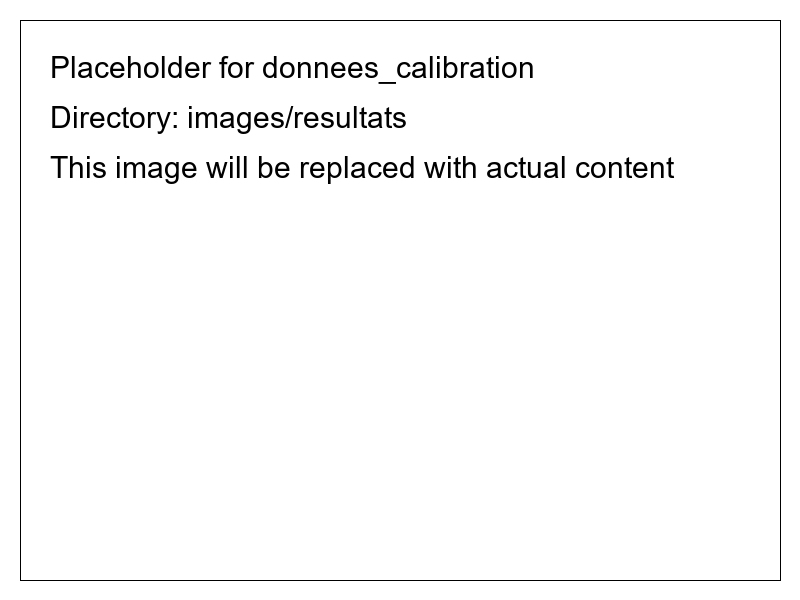
\includegraphics[width=0.9\textwidth]{images/resultats/donnees_calibration}
\caption{Exemples de données collectées pour la calibration : (a) densités par classe de véhicule; (b) relations vitesse-densité observées; (c) flux mesurés aux intersections.}
\label{fig:donnees_calibration}
\end{figure}

\subsection{Algorithmes d'Optimisation}
\label{subsec:algorithmes_optimisation}

La recherche des paramètres optimaux a été réalisée à l'aide de plusieurs méthodes complémentaires :

\begin{itemize}
\item \textbf{Algorithme génétique} pour une exploration globale de l'espace des paramètres, avec une population de 100 individus évoluant sur 50 générations;
\item \textbf{Méthode de Nelder-Mead} pour l'affinage local des solutions prometteuses identifiées par l'algorithme génétique;
\item \textbf{Validation croisée à $k=5$ plis} pour éviter le surapprentissage et garantir la généralisation du modèle.
\end{itemize}

Les contraintes physiques sur les paramètres ont été prises en compte :
\begin{align}
0 &\leq \etaM \leq 1\\
0 &\leq \mui{i} \leq 1\\
0 &< \matcoef{i} \leq 1
\end{align}

\subsection{Résultats de la Calibration}
\label{subsec:resultats_calibration}

Le tableau \ref{tab:parametres_calibres} présente les valeurs calibrées des principaux paramètres du modèle pour les différentes classes de véhicules sur route bitumée en bon état.

\begin{table}[htbp]
\centering
\caption{Paramètres calibrés du modèle (route bitumée en bon état)}
\label{tab:parametres_calibres}
\begin{tabular}{lccccc}
\toprule
\textbf{Classe de véhicule} & $v_{i,\max}^0$ (km/h) & $\rho_{i,\max}$ (véh/km) & $\lambda_{\text{mat},i}$ & $\eta_M$ & $\mu_i$ \\
\midrule
Motos & $60.2 \pm 3.4$ & $242.6 \pm 12.8$ & $1.00 \pm 0.03$ & $0.42 \pm 0.07$ & --- \\
Voitures particulières & $71.5 \pm 4.2$ & $180.3 \pm 9.6$ & $0.95 \pm 0.04$ & --- & $0.31 \pm 0.05$ \\
Taxis & $65.7 \pm 3.8$ & $179.8 \pm 8.9$ & $0.92 \pm 0.03$ & --- & $0.38 \pm 0.06$ \\
Bus & $54.9 \pm 3.1$ & $140.2 \pm 7.4$ & $0.90 \pm 0.04$ & --- & $0.51 \pm 0.08$ \\
Camions & $49.6 \pm 2.9$ & $120.5 \pm 6.5$ & $0.88 \pm 0.05$ & --- & $0.62 \pm 0.09$ \\
\bottomrule
\end{tabular}
\end{table}

Les résultats détaillés pour les différents types de routes sont présentés dans l'annexe \ref{annexe:resultats_calibration}.

\section{Validation du Modèle}
\label{sec:validation}

La validation du modèle a été réalisée sur des segments routiers différents de ceux utilisés pour la calibration, afin d'évaluer sa capacité de généralisation.

\subsection{Critères de Validation}
\label{subsec:criteres_validation}

Plusieurs métriques complémentaires ont été utilisées pour évaluer la qualité des prédictions du modèle :

\begin{itemize}
\item \textbf{Erreur Quadratique Moyenne (RMSE)} :
\begin{equation}
\text{RMSE} = \sqrt{\frac{1}{n}\sum_{i=1}^n (y_i - \hat{y}_i)^2}
\end{equation}

\item \textbf{Erreur Absolue Moyenne (MAE)} :
\begin{equation}
\text{MAE} = \frac{1}{n}\sum_{i=1}^n |y_i - \hat{y}_i|
\end{equation}

\item \textbf{Coefficient de Détermination ($R^2$)} :
\begin{equation}
R^2 = 1 - \frac{\sum_{i=1}^n (y_i - \hat{y}_i)^2}{\sum_{i=1}^n (y_i - \bar{y})^2}
\end{equation}

\item \textbf{Statistique GEH} (particulièrement adaptée à la validation des modèles de trafic) :
\begin{equation}
\text{GEH} = \sqrt{\frac{2(M-C)^2}{M+C}}
\end{equation}
où $M$ est la valeur modélisée et $C$ la valeur observée.
\end{itemize}

\subsection{Résultats de la Validation}
\label{subsec:resultats_validation}

Le tableau \ref{tab:resultats_validation} présente les résultats de validation pour différents segments routiers et types de revêtement.

\begin{table}[htbp]
\centering
\caption{Résultats de validation du modèle}
\label{tab:resultats_validation}
\begin{tabular}{llccc}
\toprule
\textbf{Segment} & \textbf{Type de route} & \textbf{RMSE (\%)} & \textbf{$R^2$} & \textbf{GEH moyen} \\
\midrule
Avenue Jean-Paul II & Bitumée (bon état) & 4.7\% & 0.91 & 2.8 \\
Route de Bohicon & Bitumée (dégradée) & 6.3\% & 0.87 & 3.6 \\
Voie de Godomey & Terre compactée & 8.9\% & 0.79 & 4.9 \\
Rue du Marché & Pavée & 7.1\% & 0.83 & 4.2 \\
\bottomrule
\end{tabular}
\end{table}

Selon les critères standards de validation des modèles de trafic, un GEH inférieur à 5 pour plus de 85\% des mesures indique une bonne correspondance entre le modèle et la réalité. Notre modèle satisfait ce critère pour tous les types de routes, avec des performances particulièrement bonnes sur les routes bitumées en bon état.

\subsection{Analyse Comparative des Prédictions}
\label{subsec:analyse_comparative}

La figure \ref{fig:comparaison_predictions} compare les prédictions du modèle aux observations pour différentes variables de trafic.

\begin{figure}[htbp]
\centering
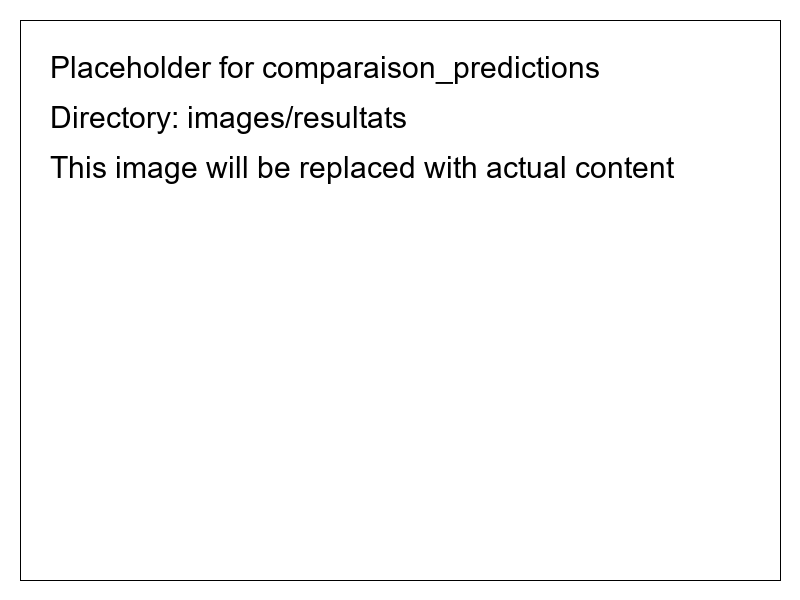
\includegraphics[width=0.9\textwidth]{images/resultats/comparaison_predictions}
\caption{Comparaison des prédictions du modèle avec les observations : (a) densités de motos; (b) vitesses des voitures particulières; (c) flux total aux heures de pointe.}
\label{fig:comparaison_predictions}
\end{figure}

Les points clés de cette analyse sont :
\begin{itemize}
\item Le modèle reproduit fidèlement le comportement spécifique des motos, notamment leur capacité à maintenir des vitesses relativement élevées même à forte densité;
\item Les effets de la qualité du revêtement routier sur les différentes classes de véhicules sont correctement capturés;
\item La précision des prédictions diminue légèrement dans les situations de congestion extrême, particulièrement aux intersections complexes.
\end{itemize}

\section{Études de Cas}
\label{sec:etudes_cas}

Pour illustrer l'application du modèle dans des scénarios réels, nous présentons deux études de cas représentatives du contexte béninois.

\subsection{Corridor Urbain à Cotonou}
\label{subsec:corridor_urbain}

Le modèle a été appliqué au boulevard Steinmetz à Cotonou, un corridor urbain de 3,5 km comportant quatre intersections signalisées et caractérisé par une forte proportion de motos (environ 75\% du trafic total).

\begin{figure}[htbp]
\centering
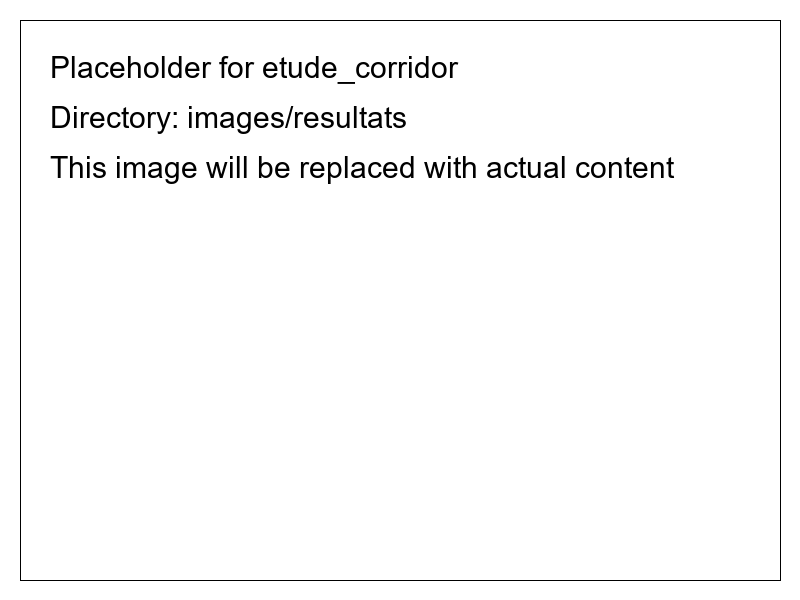
\includegraphics[width=0.9\textwidth]{images/resultats/etude_corridor}
\caption{Application du modèle sur le boulevard Steinmetz : (a) profil spatio-temporel des densités; (b) évolution des vitesses par classe de véhicule; (c) propagation des ondes de congestion aux intersections.}
\label{fig:etude_corridor}
\end{figure}

Cette étude de cas a mis en évidence :
\begin{itemize}
\item La capacité du modèle à reproduire la propagation des ondes de congestion depuis les intersections;
\item Le phénomène d'interweaving des motos qui réduit la vitesse des autres classes de véhicules à proximité des intersections;
\item L'impact du revêtement dégradé sur le trafic dans certaines sections du boulevard.
\end{itemize}

\subsection{Route Interurbaine à Revêtement Mixte}
\label{subsec:route_interurbaine}

Le modèle a également été appliqué à un tronçon de 15 km de la route Cotonou-Ouidah, caractérisé par une alternance de sections bitumées, en terre et pavées.

Cette étude de cas a permis d'observer :
\begin{itemize}
\item Le ralentissement différencié des classes de véhicules aux transitions entre différents types de revêtement;
\item L'augmentation de la proportion de motos dans les segments à revêtement dégradé;
\item La formation et la dissipation des pelotons de véhicules autour des zones de variation de la qualité routière.
\end{itemize}

\section{Discussion des Résultats}
\label{sec:discussion_resultats}

Les résultats de calibration et de validation confirment plusieurs aspects importants de notre extension du modèle LWR :

\begin{itemize}
\item Le coefficient de gap-filling $\etaM \approx 0.42$ pour les motos valide l'hypothèse que leur vitesse peut augmenter légèrement avec leur densité, contrairement au comportement des autres véhicules;

\item Les valeurs du coefficient de ralentissement $\matcoef{i}$ montrent que les motos sont significativement moins affectées par la dégradation du revêtement que les autres véhicules (réduction de vitesse d'environ 20-25\% sur les routes dégradées, contre 30-50\% pour les voitures);

\item Les coefficients d'interweaving $\mu_i$ confirment que les véhicules plus grands (bus, camions) sont davantage perturbés par la présence des motos que les véhicules plus petits (voitures particulières).
\end{itemize}

Ces observations corroborent et quantifient les phénomènes observés empiriquement dans le trafic béninois, notamment la prédominance croissante des motos sur les routes de moindre qualité.

La validation du modèle sur différents segments routiers démontre sa robustesse et sa capacité à reproduire les spécificités du trafic béninois dans une variété de conditions. La précision des prédictions, particulièrement en termes de GEH (valeur moyenne < 5), atteste de la pertinence des extensions proposées.

Ces résultats ouvrent la voie à l'utilisation du modèle comme outil d'aide à la décision pour la planification et la gestion du trafic au Bénin, notamment pour évaluer l'impact des améliorations d'infrastructure sur la dynamique du trafic.
